\chapter{Future work}
\label{ch:closing}

This chapter describes the plan of tasks to be performed in order to complete the proposed research aim. The tasks are related to at least one research objective, which are also related to each one of the parts that compose this research. Figure \ref{fig:future-work-objectives} illustrates the parts and the research objectives whose tasks will be conducted.

\begin{figure}[h]
    \centering
    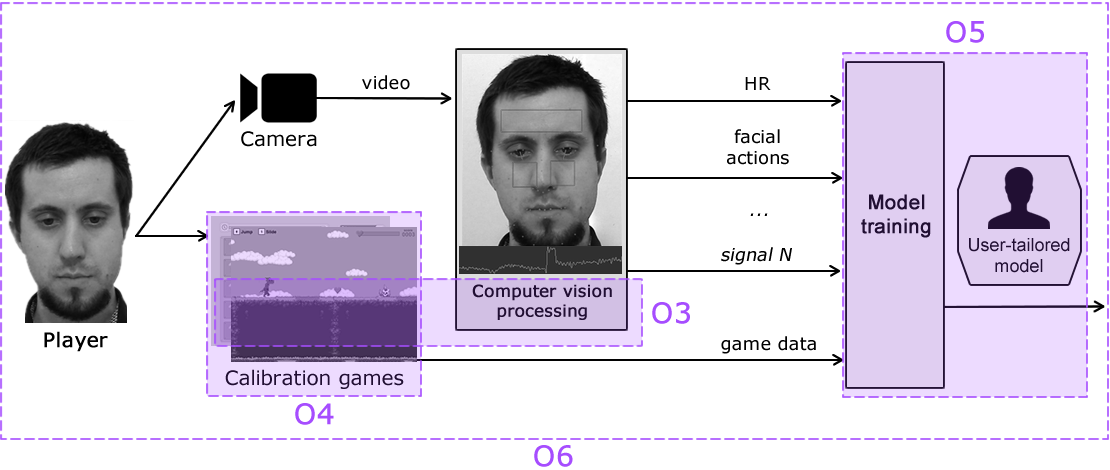
\includegraphics[width=\textwidth]{figures/future-work-objectives.png}
    \caption{Highlight of research objectives and related parts of the solution whose tasks will be conducted as future work.}
    \label{fig:future-work-objectives}
\end{figure}

The tasks involve the refinement of process of remote acquisition of signals, fefinition of inputs for the user-tailored model, investigation of machine learning models, execution of an experiment involving emotion detection, refinement of the process of user-tailored emotion detection and finally the construction of a software that uses the proposed method. The schedule below shows the time progression of the tasks. The following sections describe the tasks in detail.

\begin{landscape}

\begin{center}
\begin{tabular}{ |p{6.5cm}|c|c|c|c|c|c|c|c|c|c|c|c|c|c| }
\hline
\textbf{Activity} & \multicolumn{2}{|c|}{2015} & \multicolumn{4}{|c|}{2016} & \multicolumn{4}{|c|}{2017} & \multicolumn{4}{|c|}{2018} \\
\hline
 & 3 & 4 & 1 & 2 & 3 & 4 & 1 & 2 & 3 & 4 & 1 & 2 & 3 & 4 \\
\hline
Literature review & \cellcolor{Gray} & \cellcolor{Gray} & \cellcolor{Gray} & \cellcolor{Gray} & \cellcolor{Gray} & \cellcolor{Gray} &  &  &  &  &  &  &  &  \\
\hline
Planning and design of calibration games &  &  & \cellcolor{Gray} & \cellcolor{Gray} &  &  &  &  &  &  &  &  &  &  \\
\hline
Implementation of calibration games &  &  &  & \cellcolor{Gray} & \cellcolor{Gray} &  &  &  &  &  &  &  &  &  \\
\hline
Experiments with calibration games &  &  &  & \cellcolor{Gray} & \cellcolor{Gray} &  &  &  &  &  &  &  &  &  \\
\hline
Investigation of calibration games data &  &  &  &  & \cellcolor{Gray} & \cellcolor{Gray} &  &  &  &  &  &  &  &  \\
\hline
Identification of signals to be remotely read &  &  &  &  &  & \cellcolor{Gray} & \cellcolor{Gray} &  &  &  &  &  &  &  \\
\hline
Investigation of signals and their relation with stress/boredom &  &  &  &  &  &  & \cellcolor{Gray} & \cellcolor{Gray} &  &  &  &  &  &  \\
\hline
Planning of computer vision software &  &  &  &  &  &  &  & \cellcolor{Gray} &  &  &  &  &  &  \\
\hline
Implementation of computer vision software &  &  &  &  &  &  &  &  & \cellcolor{Gray} & \cellcolor{Gray} &  &  &  &  \\
\hline
Design of prediction model &  &  &  &  &  &  &  & \cellcolor{Gray} & \cellcolor{Gray} & \cellcolor{Gray} &  &  &  &  \\
\hline
Validation of prediction model &  &  &  &  &  &  &  &  &  &  & \cellcolor{Gray} & \cellcolor{Gray} &  &  \\
\hline
Field test with game development studio &  &  &  &  &  &  &  &  &  &  &  & \cellcolor{Gray} &  &  \\
\hline
Thesis writing &  &  &  &  &  &  &  & \cellcolor{Gray} & \cellcolor{Gray} & \cellcolor{Gray} & \cellcolor{Gray} & \cellcolor{Gray} & \cellcolor{Gray} &  \\
\hline
Disputation &  &  &  &  &  &  &  &  &  &  &  &  &  & \cellcolor{Gray} \\
\hline
\hline
\end{tabular}
\end{center}

\end{landscape}

\section{Refinement of remote acquisition of signals}

The information presented in chapter \ref{ch:literature-rppg} suggests that techniques for remote extraction of physiological signals of users are significantly affected by natural behavior, e.g. head movement and facial activity. The results of the first experiment also support that, indicating that users indeed behave in a way that directly affect the accuracy of measurements. Preliminary analysis \parencite{bevilacqua2017accuracy} suggests that the accuracy of the rPPG technique is feasable under such circustances, however it is still not clear how the accuracy problems interfer with a predictive model.

As a consequence, studies will be conducted to investigate how the selected rPPG technique are affected by the natural behavior of user and how it can be improved to mitigate or elimitate those problems. Figure \ref{fig:rppg-accuracy-study} illustrates the process to be conducted to evaluate and improve the accuracy of the rPPG technique.

\begin{figure}[h]
    \centering
    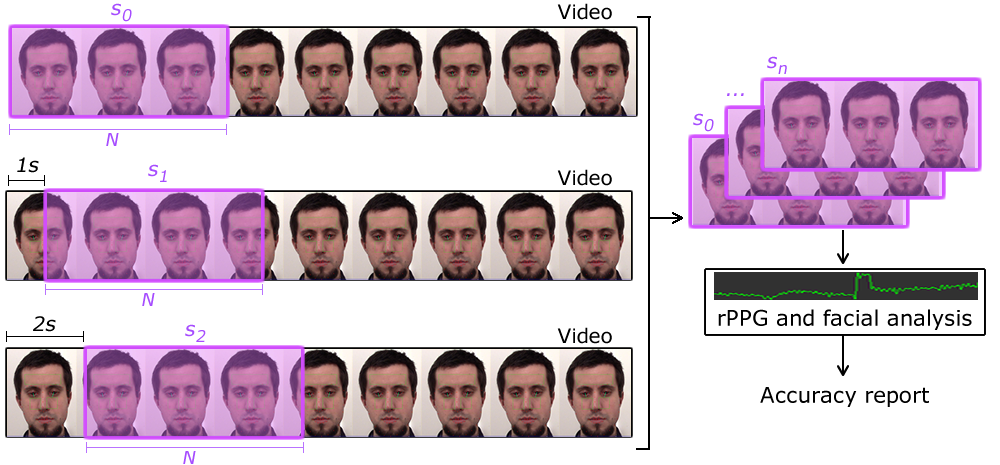
\includegraphics[width=\textwidth]{figures/rppg-accuracy-study}
    \caption{Process to evaluate the accuracy of HR estimations performed by rPPG when influenced by natural behavior.}
    \label{fig:rppg-accuracy-study}
\end{figure}

The video recordings of the first experiment will be used in the analysis. All videos will be analysed using a moving window of size $N$ seconds, which will be moved along the videos with a 1 second offset, producing a set $S$ of video segments $s_i$ with $N$ seconds each. For example, assuming a 1 minute long video and a 30 seconds moving window ($N=30$), the analysis process will result in 30 $s_i$ segments ($S=30$) of 30 seconds each (0 to 30, 1 to 31, ..., 29 to 59).

Each segment $s_i$ will be used as the input for the rPPG technique for HR estimation. The estimated HR value will be compared to the average HR calculated from ground truth for the duration of the segment $s_i$. Additionally facial movement information will be calculated for each segment, such as variations of ROI size, ROI position the and variations of the central point of the detected face. Similar calculations were already conducted in study 3 (section \ref{s:study3}).

Different values for the window size $N$ will be used in the analysis, which will identify a correlation among the size of $N$, the effect of user movements and the accuracy of HR estimations. Those values will guide the adaptations proposed by previous work \parencite{li2014remote} to be applied into the selected rPPG technique to improve its accuracy within the context of this research.

\section{Definition of inputs for the user-tailored model}
\label{sec:closing-definition-inputs}

The literature presented in chapters \ref{ch:literature-physiological}, \ref{ch:literature-face} and \ref{ch:literature-multifactorial} indicates that a model based on several user signals, which is a multifactorial analysis, is more efficient for emotion detection. The mentioned chapters also highlight which of those signals can be remotely acquired within the context of this research via computer vision techniques.

\begin{figure}[h]
    \centering
    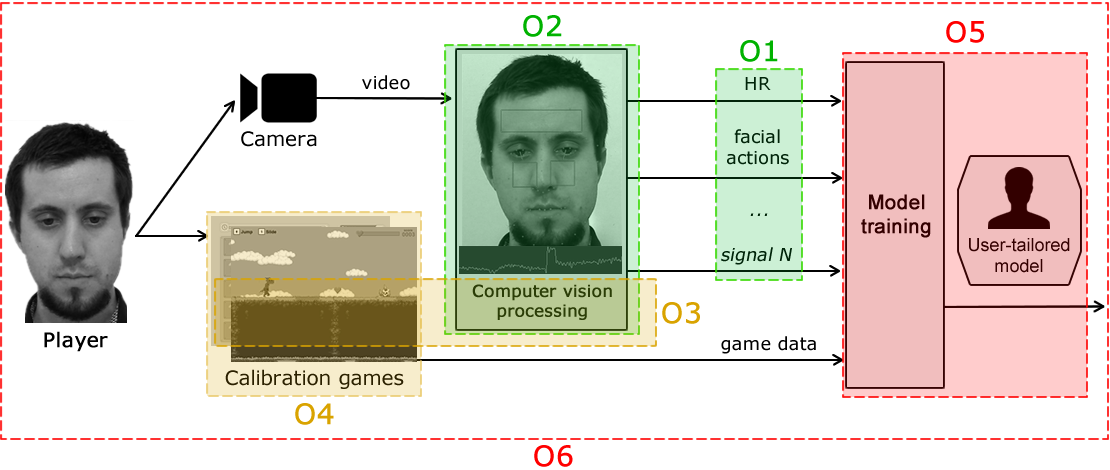
\includegraphics[width=\textwidth]{figures/components-objectives.png}
    \caption{Input user-tailored model}
    \label{fig:model-input-definition}
\end{figure}

The user-tailored model proposed for this research might have $N$ input signals, varying from physiological ones, e.g. HR, to non-physiological ones, e.g. facial actions and head movements. Figure \ref{fig:model-input-definition} illustrates the process. Each one of those signals, however, needs to be supported by previous work regarding emotion detection, as well as be validated within the process of the proposed game-based calibration phase. Time and scope constraints limit the amount of input signals that can be implemented, evaluated and used in this research. As a consequence, a study will be conducted to investigate, validate and initially implement two of those signals into the proposed model: HR and facial activity (which includes head movement, lips activity, etc).

The techniques and works presented in chapter \ref{ch:literature-face}, which relate to face detection and emotion estimation, suggest that facial analysis is an important component of a multifactorial emotion detection model. Empirical analysis of the data from the first experiment also suggest that individualities regarding facial activities do exist and could be used to estimate emotional states on a user-tailored basis \parencite{bevilacqua2016variations}. As described in section \ref{ch:literature-face-emotion-prediction}, facial actions, head movement, lips/eye/mouth activity and distance measurements of detected facial landmarks are viable and proved sources of information for emotion detection.

Regarding physiological signals, results indicate that the average HR mean for players during the last minute of gameplay is greater than the average HR mean during the second minute of gameplay. The findings are aligned with and reinforce previous research that indicate higher HR mean during stressful situations in a gaming context. The findings also suggest that changes in the HR during gaming sessions is a promising indicator of stress.

The study will involve the definition of how those two signals will be used as inputs for the model. Facial actions will be detected and measured by the euclidian distance of the facial landmarks. A vector containing the distances will be evaluated as the input for the model. Regarding the HR, its mean and standard variation during a particular analysis window will be evaluated as input for the model. A software for the detection of those two signals will be created and used to analyse the video recordings of the first experiment. The inclusion or exclusion of a component of a signal, e.g. variations of the distances of the lips landmark points, will be based on the accuracy to detect them and the frequency they appear in boring and stressful part of the calibration games.

\section{Investigation of machine learning models}
\label{closing:investigation-machine-learning}

The majority of the previous work found in the literature mention the use of machine learning models to map user signals into emotional states. Different models and accuracy results are mentioned, which dependent on several particularities of the approach used by the authors. A machine learning model will also be used by this research as a user-tailored emotion detection model.

\begin{figure}[h]
    \centering
    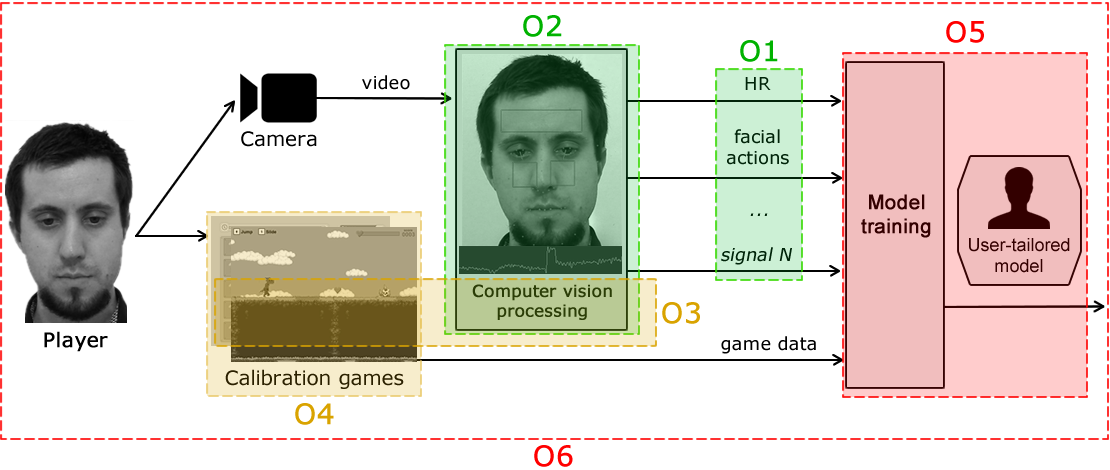
\includegraphics[width=\textwidth]{figures/components-objectives.png}
    \caption{machine-learning-investigation}
    \label{fig:machine-learning-investigation}
\end{figure}

A systematic study and accuracy evaluation will be performed to select the proper machine learning technique to be used in the model. The evaluation process, illustrated in Figure \ref{fig:machine-learning-investigation}, will be conducted on each one of the selected (and competing) machine learning techniques using the video recordings of experiment 1. The evaluation is based on a 3 fold cross validation process. Initially the input signals for the emotion detection model (defined in the previous tasks, section \ref{sec:closing-definition-inputs}) will be extracted from two of the three games played by a user and used to train the emotion detection model. The thrid game that was left out of the training will be used as a testing set: user signals will be extracted and fed into the trained emotion detection model, which will output the predicted emotional state of the user. The 3 fold cross validation process is repeated three times, each one of them leaving a different game out of the training phase.

The video recordings that will be used in the tasks are related to experiment 1, whose games were designed to work as calibration games. As previously described in section \ref{sec:research-aim}, those calibration games feature a progression from a boring to a stressful state. That configuration will be used as the foundation for the labeling process of emotional states during the training of the model, as well as ground truth for its testing.

\begin{figure}[h]
    \centering
    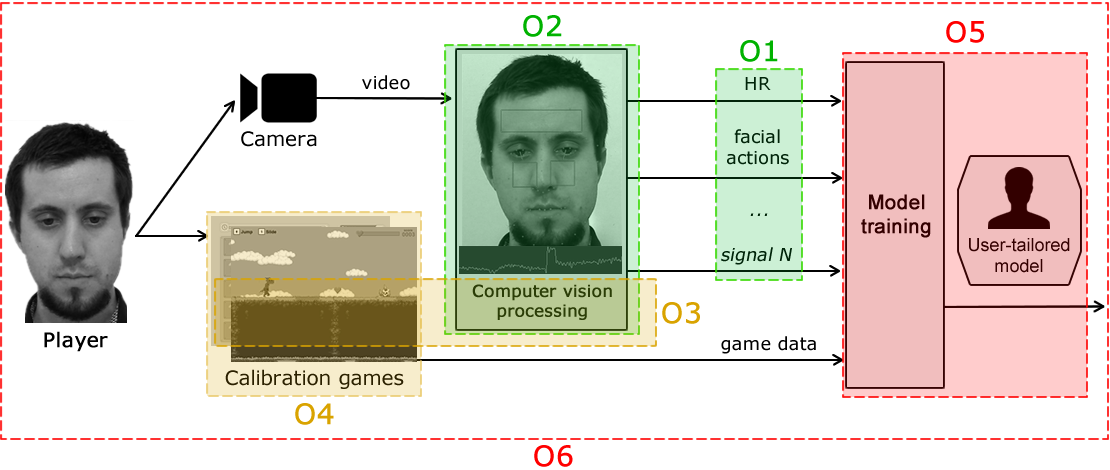
\includegraphics[width=\textwidth]{figures/components-objectives.png}
    \caption{machine-learning-labeling-approach}
    \label{fig:machine-learning-labeling-approach}
\end{figure}

The training of the emotion detection model will be conducted according to two different strategies illustrated in Figure \label{fig:machine-learning-labeling-approach}. In both approaches, the two games used as training sets will have their user signals sampled at a fixed interval of $T$ seconds, being $T$ empirically defined. The labeling of the sample as boredom or stress, however, will be different. In approach \textbf{A}, assuming that $P$ represents the time progression of each game, e.g. $P=0$ is the starting point of the game and $P=1$ is its end point, each game will be divided in two equal parts ($P=0.5$). Samples from the first half of the game will be labeled as boredom, while samples from the second half will be labeled as stress. The division is based on the assumption that the middle of the games accurately separates in time the self-reported perceptions of boredom and stress made by the subjects. In approach \textbf{B}, the self-reported levels of boredom and stress associated with the beginning and the end of each game will be used. Assuming that $S_i$ and $B_i$ represent the self-reported stress and boredom levels of a given subject, respectively, where $i=0$ represents the beginning part of a game, and $i=1$ represents the ending part of a game. Two distinc division points will be calculated for boredom and stress labelings. The division point for stress, $P_s$, will be calculated as:

\begin{equation}
P_s = 1 - \frac{S_1 - S_0}{5}
\end{equation}

and the division point for boredom, $P_b$, will be calculated as:

\begin{equation}
P_b = \frac{B_1 - B_0}{5}
\end{equation}

where 5 is the maximum value allowed for the self-reported answers. The values of $P_s$ and $P_b$ will range within the interval [0,1], which will be used as the division point similarly to the one described for approach \textbf{A}. For example, a subject that reported $S_0=0$ and $S_1=5$ will have $P_s=0.5$ (middle point of the game), while a subject with $S_0=3$ and $S_1=4$ will have $P_s=0.8$. Samples from the second half of the division $P_s$ will be labeled as stress, while the samples from the first half of $P_b$ will be labeled as boredom.

The testing process will be similar for both approaches \textbf{A} and \textbf{B}. Samples from the game used as a testing set will be collected at a fixed internal of $K$ seconds, which will be larger than $T$ and also defined empirically. The associated labeling of the samples will be based on their position in the two parts calculated according to the rules of division points for each approach. Sample points that eventually are not labeled, e.g. middle points in approach \textbf{B}, will be labeled as neutral.

Following the described procedure, after all machine learning techniques are tested, they will have several resulting accuracy scores, i.e. $3 \cdot K \cdot 20$, where 20 is the number of subjects of experiment 1. The technique with the highest mean for the accuracy score will be selected. The following machine learning and classification techniques will be initially used in the tests: Support Vector Machine (SVM) using a radial basis, C-Support Vector Classification (C-SVC) using a linear kernel, K-nearest neighbours (K-nn), AdaBoost using nearest mean classifiers, Naive Bayers, and neural networks probably represented by convolution networks (convnets). Previous work also suggest a process involving decision fusion or a hierarchy of two or more classifiers working on different feature sets to improve prediction rates. Those approaches will probably be investigated as well.

\section{Emotion detection experiment}
\label{closing:emotion-detection-experiment}

After the machine learning technique has been selected and the inputs for the model have been defined, a new experiment will be conducted. The experiment will be similar to the first one conducted, however it will test the hypotesis that all defined components, i.e. computer vision technique, machine learning model and calibration games, work in combination to detect emotional states.

The experiment design will be based on a within-subject approach \cite{lane2015online} where all participants perform at all levels of the treatment and there are no control groups. In the context of this research, user signals, e.g. HR, facial actions and self-reported emotional state, will be measured and used in a user-tailored model, so the division of subjects into more than one group poses a comparison problem. Each individual will inevitably differ from one another regarding signals and emotions, such as variations in average HR during rest, for instance. Additionally the emotional state of users regarding boredom and stress must be measured constantly during the experiment, so the accuracy of the user-tailored model can be tested against those points where the emotional state is known.

\begin{figure}[ht]
    \centering
    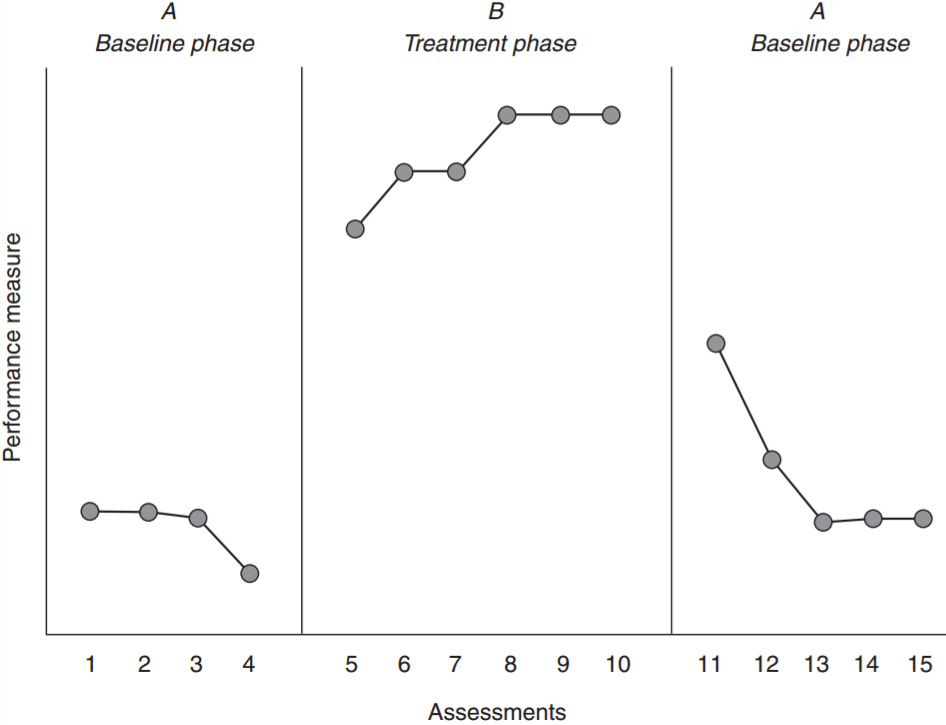
\includegraphics[scale=0.5]{figures/time-series-design-breakwell.png}
    \caption{\textcite{breakwell1994research}}
    \label{fig:time-series-design-breakwell}
\end{figure}

Since the emotional state of users must be measured constantly, a time-series experimenta design will be used. In a time-series design there is a presence of a periodic measurement process on an individual and the introduction of an experimental change into this time series of measurements, which results in a discontinuity in the measurements recorded in the time series \textcite{campbell2015experimental}. Figure \ref{fig:time-series-design-breakwell} illustrates the design. The A-B-A design is a common single-case experimental design in which the measurements are conducted throughout the three parts of the experiment, i.e. A, B and A. Phase A, referred to as the baseline phase, is a period where the subject is not under the effect of the treatment, so the measurements should reflect natural occurences. Phase B, referred as the treatment phase, is the period where the treatment/intervention is applied. In the A-B-A design, the application of a treatment followed by its removal should result in changes in the measurements among the three phases, e.g. lower values during phase A and elevated values during phase B, which confirms that the variation is a result of the treatment.

The experiment will use a multiple treatment design which involves the implementation of two or more treatments designed to affect a single behavior \parencite{robson2016real}. It will have the form of A-B-A-C-A-D-A, where B, C and D are treatments. In the experiment, treatments B and C will be calibration games, while treatment D will be an ordinary off the shelf game. Figure \ref{fig:closing-experiment2-design} illustrates the design of the experiment.

\begin{figure}[ht]
    \centering
    \includegraphics[scale=0.5]{figures/experiment-design.png}
    \caption{One-group posttest experiment design used in this research. $S_j$ represents the $j^{\text{th}}$ subject, $G_i$ represents a game of type $i$, $PT_i$ is the post-test for game $G_i$ and $rest$ is a resting period.}
    \label{fig:closing-experiment2-design}
\end{figure}

Two calibration games, named $G_1$ and $G_2$, will be selected as treatments. The order they will be played will be randomized among participants, so one subject will have $G_1$ for treatment B and $G_2$ for treatment C, while another subject will have $G_2$ for B and $G_1$ for C, and so on. The measurement to be conducted will be regarding the levels of stress and boredom. At fixed intervals, e.g. every 60 seconds, users will be asked to report the current emotional state. The measurement mechanism will be defined, however it will be one of the following options. A likert scale containing a question about the stress level and a question about the boredom level. The Self-Assessment Manikin (SAM) \parencite{morris1995observations}, which is an efficient cross-cultural measurement of emotional response regarding valence and arousal. Or the Affective Slider (AS) \parencite{betella2016affective}, a digital self-reporting tool composed of two slider controls for assessment of pleasure and arousal. Figure \ref{fig:sam-as} illustrates both self-assessment mechanisms.

\begin{figure}[h]
\centering
  \begin{subfigure}[b]{0.5\textwidth}
    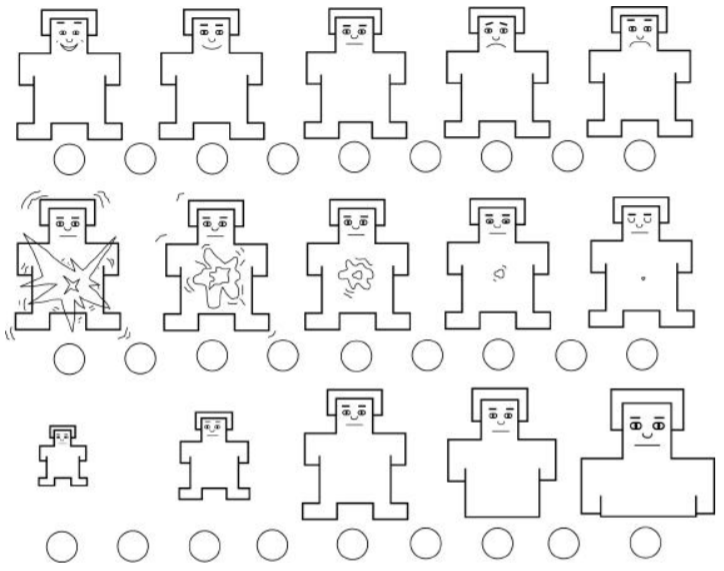
\includegraphics[width=0.95\textwidth]{figures/SAM.png}
    \caption{}
    \label{fig:sam}
  \end{subfigure}%
  \begin{subfigure}[b]{0.5\textwidth}
    \centering
    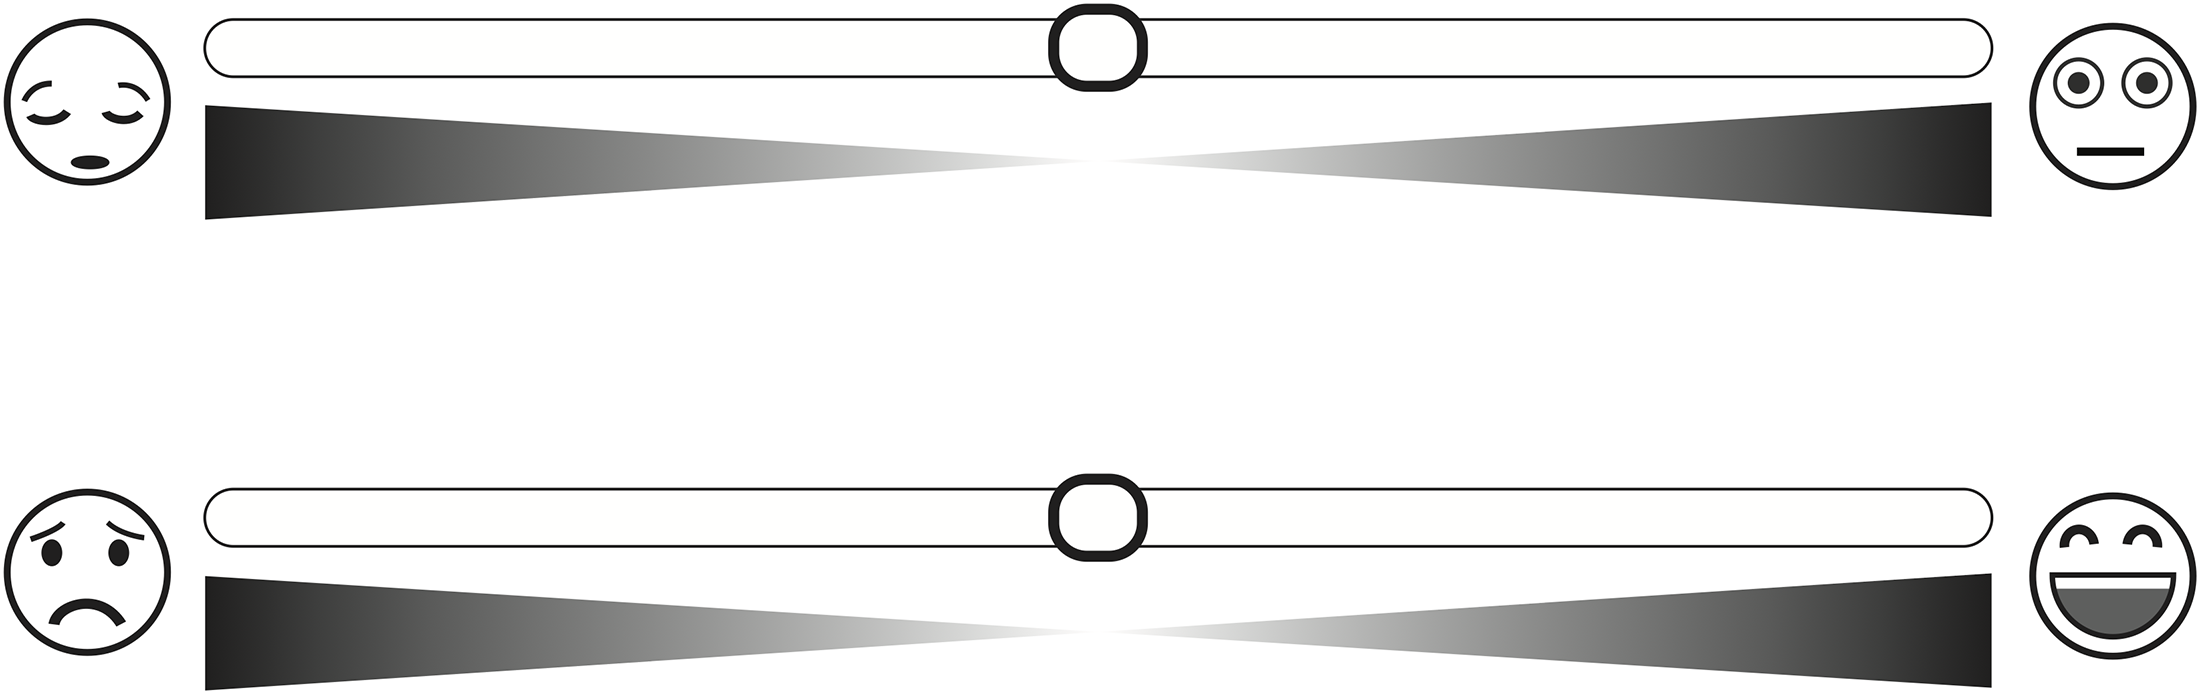
\includegraphics[width=0.95\textwidth]{figures/AS.png}
    \caption{}
    \label{fig:as}
  \end{subfigure}
  \caption{Self-reporting meaurement of emotional states. (a) Self-Assessment Manikin (SAM) \parencite{morris1995observations}; (b) Affective Slider (AS) \parencite{betella2016affective}.}
  \label{fig:sam-as}
\end{figure}

Additionally to the self-assessment of the emotional state, during the whole experiment subjects will be recorded by a video camera and monitored by a HR watch. The data collected during the experiment regarding the calibration games will be used to train a machine learning model, which will be used to detect the emotional state of users during the interaction with the ordinary game. Results of that analysis will prove or refute the previously mentioned hypothesis that all defined components, i.e. computer vision technique, machine learning model and calibration games, work in combination to detect emotional states.

%When measuring HR, for instance, some subjects will have higher/lower HR mean than others, independent of the group they are in or the treatment they undergo. To counter that problem, the experiment will use a one-group posttest design \cite{kirk1982experimental}, as illustrated by Figure \ref{fig:closing-experiment2-design}. Using the first row as an example, subject $S_0$ played game $G_a$ as the first level of the treatment, followed by a post-test of that game ($PT_a$), then a rest period. In the second level of the treatment, the subject played game $G_b$, followed by a post-test of that game ($PT_b$), then another rest period. Finally in the third level of the treatment, the subject played game $G_c$ followed by a post-test of that game ($PT_c$).

%By using a one-group posttest design, each individual will perform on all levels of the treatment (play a set of different games). The within-subjects approach ensures that the differences between subjects are not interfering in the comparison, since a subject is being compared to his/herself in the different levels of the treatment. Subjects are not being compared among each other. In essence, each subject is serving as his/her own control group. According to Kirk \cite{kirk1982experimental}, the one-group posttest design should only be used when the researcher knows the mean value of the independent variable when no treatment is in effect. Such information will be obtained during the resting periods of the experiment, where the baseline value for all measured signals can be established for each subject.

%The process of sampling a group of participants for each experiment will follow the convenience sampling approach, a non-probability sampling technique where participants are recruited because of their convenient accessibility/proximity to the researcher. Volunteers will be randomly recruited for each experiment. A probability sampling approach, where each individual of the population has an equal chance of being selected, would be ideal and would strength the external validity of the research. However the costs, logistics and time constraints associated with it makes such approach impractical in the context of this research.

\section{Refinement of user-tailored emotion detection model}

This tasks comprehends another iteration in the research of orchestrating and validating the remote acquisition of signals, machine learning models and calibration games. The results of previously described tasks (sections \ref{sec:closing-definition-inputs}, \ref{closing:investigation-machine-learning} and \ref{closing:emotion-detection-experiment}) should better clarify the relation among input signals and emotional states, as well as how they can be mapped using a machine learning model.

The goal of this tasks is to iterate on the data collected from experiment 1 and 2 to refine the inputs to be used in the emotion detection model. The process will be similar to the work described in section \ref{closing:investigation-machine-learning}, where a machine learning model was selected based on its accuracy. The set of the features that are remotely obtained via computer vision will be re-evaluated as input for the emotion detection mode based on the findings of experiment 2. The machine learning model used for the mapping process will also be re-evaluated in a process similar to the one described in section \ref{closing:investigation-machine-learning}. The data used for training and testing of the model, however, will be directly based on the data points collected from the time series in experiment 2. Those data points contain information regarding the emotional state of users at specific points in time, which was not the case of the data points of experiment 1. Figure \ref{fig:closing-refinment-specific-points} illustrates such differences. The data from experiment 1 contained information regarding emotional states at key moments in the game, e.g. beginning, middle and end, however those points are limited to perceptions of time, e.g. a subject can understand that the end part of a game lasts for 10 seconds, while another subject might understand it as lasting for 2 minutes. Data from experiment 2, in the other hand, are bound to time marks, e.g. questionnaire every 60 seconds, so they present a better representation of emotional states throughout the gaming session. As a consequence, both the training and testing of the machine learning model can be oriented towards those points instead of relying on assumptions, i.e. the middle point of a game session produces a part representing boredom and another representing stress.

\begin{figure}[ht]
    \centering
    \includegraphics[scale=0.5]{figures/experiment-design.png}
    \caption{fig:closing-refinment-specific-points}
    \label{fig:closing-refinment-specific-points}
\end{figure}

A systematic refinement the machine learning model will be performed following the structure previously described in \ref{closing:investigation-machine-learning}. The training and testing of the model will not be based on samples collected with a division point $P$, instead they will be based on the points of the time series obtained from experiment 2. Figure \ref{fig:closing-around-time-series} illustrates the new training and testing approach. Samples immediately preceeding and following an emotional state point by $V$ seconds will be used for the training process. A value of 15 seconds for $V$ means that all the samples within 30 seconds (15 seconds before the point, 15 seconds after it) of a point will be used for training. The value of $V$ will be empirically defined.

\begin{figure}[ht]
    \centering
    \includegraphics[scale=0.5]{figures/experiment-design.png}
    \caption{fig:closing-around-time-series}
    \label{fig:closing-around-time-series}
\end{figure}

The testing of the model will also be based on the points of the time series. In the 3 fold cross validation process, the game being used as a testing set will have its points of the time series as inputs to the model. Since the emotional state of those points is known, the accuracy evaluation of the model will be more precise, providing more information regarding which adaptations and refinements are necessary.

The cycle involving training, testing and refining the model will be conducted until the model presents acceptable accuracy results. This tasks will probably involve the refinement of input signals, as the process described in section \ref{sec:closing-definition-inputs}.

\section{Software deployment}

Finally when the emotion detection process is tested and validated, it will be deployed as a technological solution in the form of a software. All previously described tasks involve the implementation of algorithms to remotely extract the signals and to classify them using machine learning. All those steps will be coded in Matlab to provide fast iteration and to ensure scientific valididy with previous work.

This tasks involves the translation of all those developed parts, i.e. computer vision extraction of signals, processing of signals and mapping using machine learning, into a usable software. Since each of those parts have already been validated, the software can be seen as an encapsulation of those parts, which results in a valided usable solution. The software will be developed using OpenCV and C++.

%Questionnaires and physiological measurements are the most common approach used to obtain data for emotion estimation in the field of HCI and games research. Both approaches interfere with the natural behavior of users, which affects any research procedure. Initiaties based on computer vision and remote extraction of user signals for emotion estimation exist, however they are limited. Experiments of such initiatives were performed under extremely controlled situations with few game-related stimuli. Users had a passive role with limited possibilities for interaction or emotional involvement, differently than game-based emotion stimuli, where users take an active role in the process, making decision and directly interacting with the media. Previous works also focus on predictive models based on a group perspective. As a consequece, a model is usually trained from data of several users, which in practice describes the average behavior of the group, excluding or diluting key individualities of each user. In that light, there is a lack of initiatives focusing on non-obtrusive, user-tailored emotion detection models, in particular regarding stress and boredom, within the context of games research that are based on emotion data generated from game stimuli.

%After the rPPG technique has been improved and the facial analysis has been structured, a fourth study will be conducted on the data of the first experiment. It will guide the process of refining the remote detection of physiological signals along with facial analysis, which is the foundation for the predictive model proposed in this thesis. At the present moment, the software required to perform such study is almost finished and ready to be deployed. The results of this study should lead to another publication, which will describe the improvements applied to the rPPG technique and how they affect remote estimation of physiological signals.
